\documentclass[../AnalysisNoteJBuxton.tex]{subfiles}
\begin{document}

\subsubsection{\texorpdfstring{$\Lambda$K$^{-}$}{TEXT} Residuals}
\label{Residuals_LamKchM}

\begin{figure}[h]
  \centering
  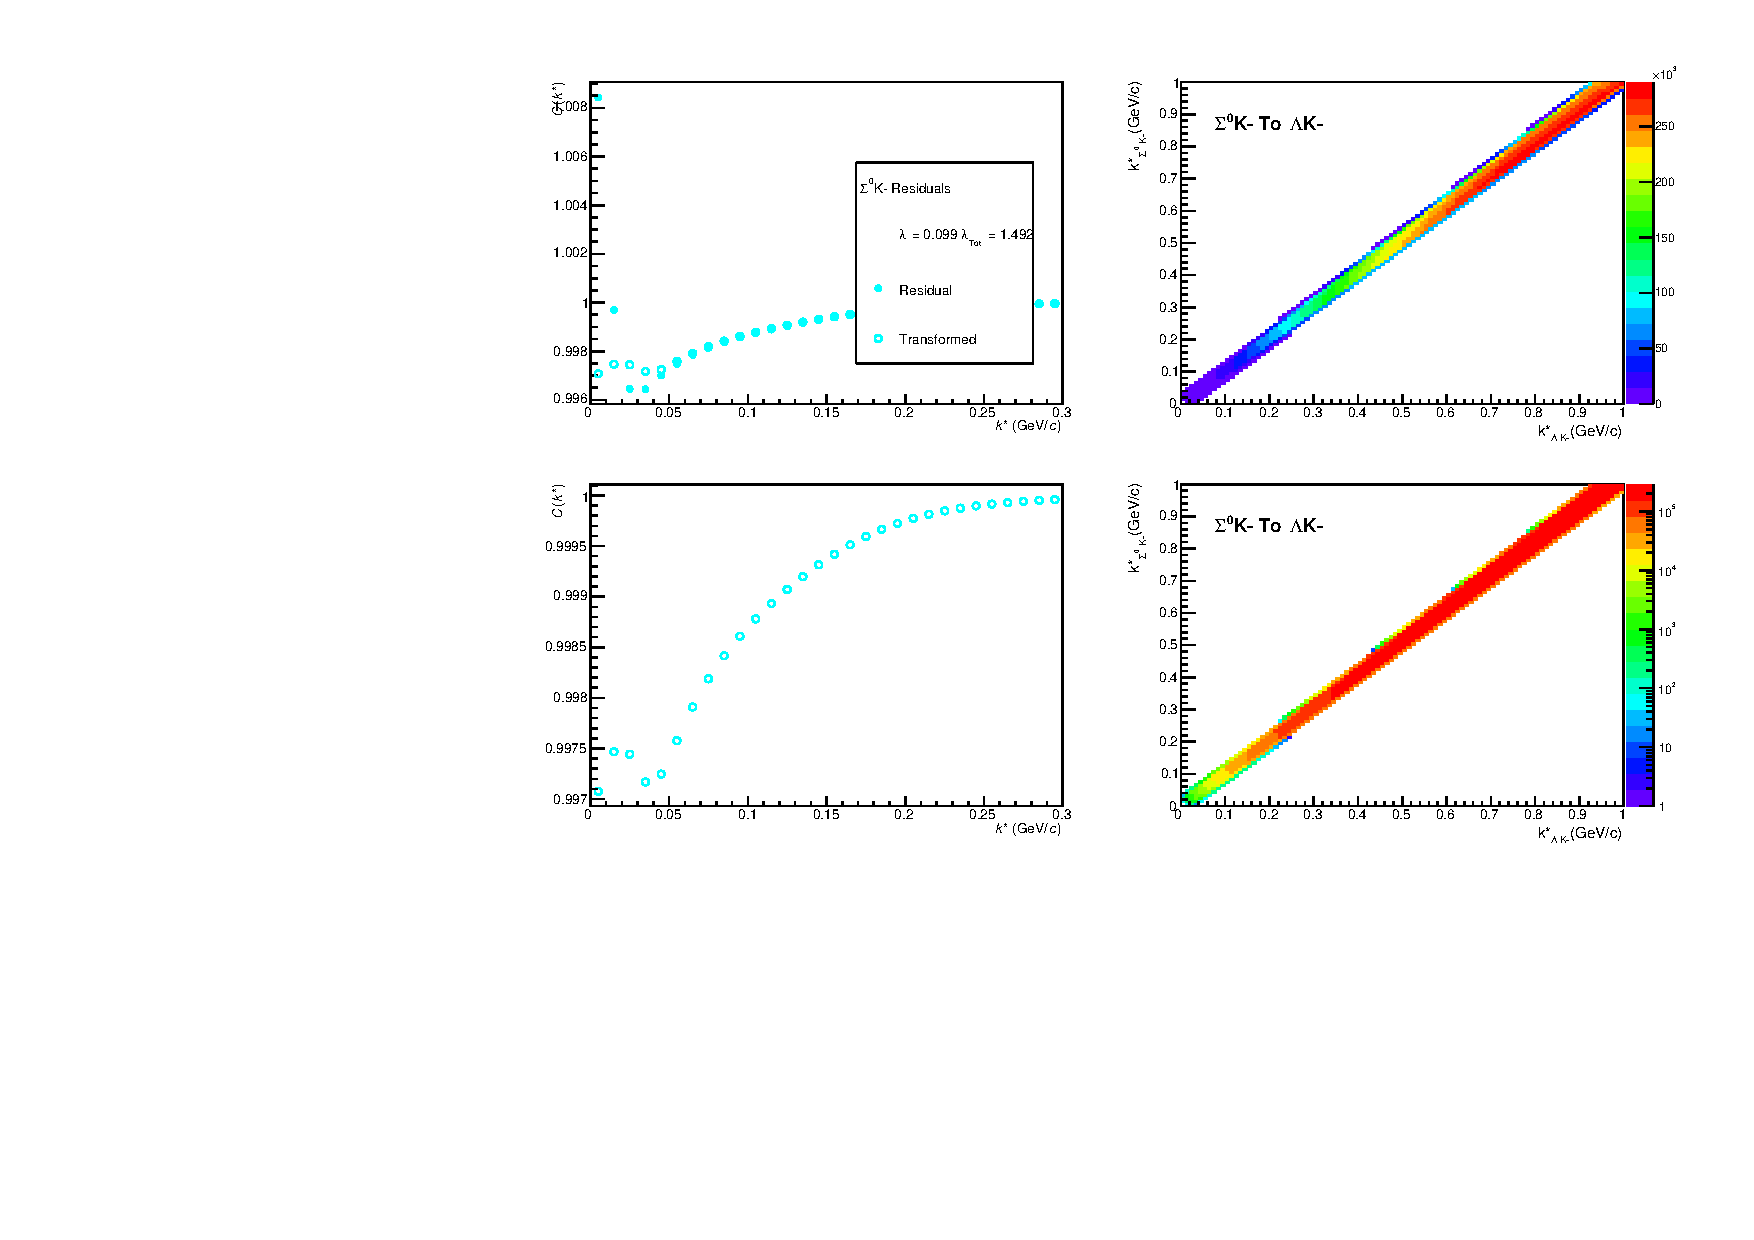
\includegraphics[width=\textwidth]{9_AdditionalFigures/Figures/Residuals/LamKchM/Residuals_LamKchM_0010_Sig0KchM_MomResCrctn_NonFlatBgdCrctn_ResidualsIncluded_UsingCoulombOnlyInterpCfs.pdf}
  \caption[Residuals: $\Sigma^{0}$K$^{-}$ to $\Lambda$K$^{-}$ (0-10\% Centrality)]{Residuals: $\Sigma^{0}$K$^{-}$ to $\Lambda$K$^{-}$ (0-10\% Centrality)}
  \label{fig:Res_LamKchM_0010_Sig0KchM}
\end{figure}


\begin{figure}[h]
  \centering
  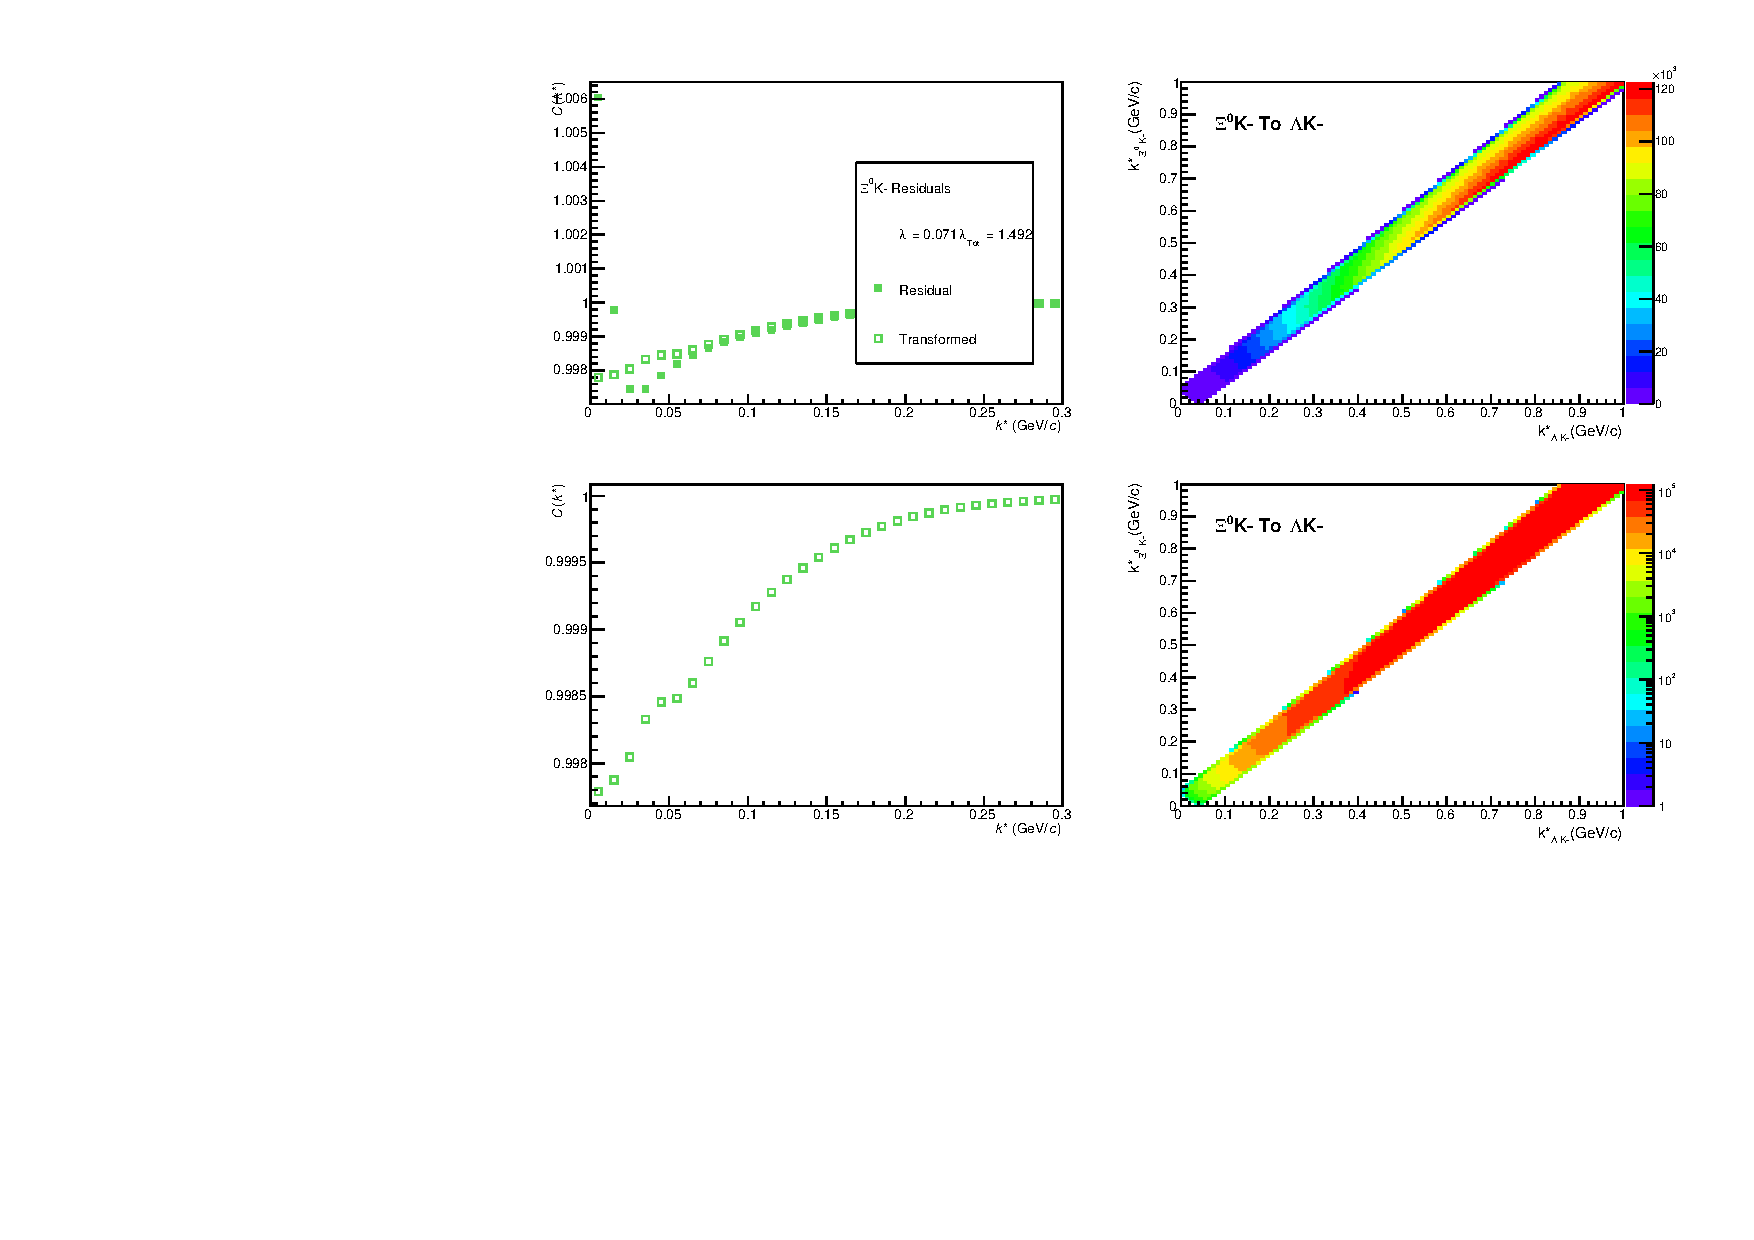
\includegraphics[width=\textwidth]{9_AdditionalFigures/Figures/Residuals/LamKchM/Residuals_LamKchM_0010_Xi0KchM_MomResCrctn_NonFlatBgdCrctn_ResidualsIncluded_UsingCoulombOnlyInterpCfs.pdf}
  \caption[Residuals: $\Xi^{0}$K$^{-}$ to $\Lambda$K$^{-}$ (0-10\% Centrality)]{Residuals: $\Xi^{0}$K$^{-}$ to $\Lambda$K$^{-}$ (0-10\% Centrality)}
  \label{fig:Res_LamKchM_0010_Xi0KchM}
\end{figure}


\begin{figure}[h]
  \centering
  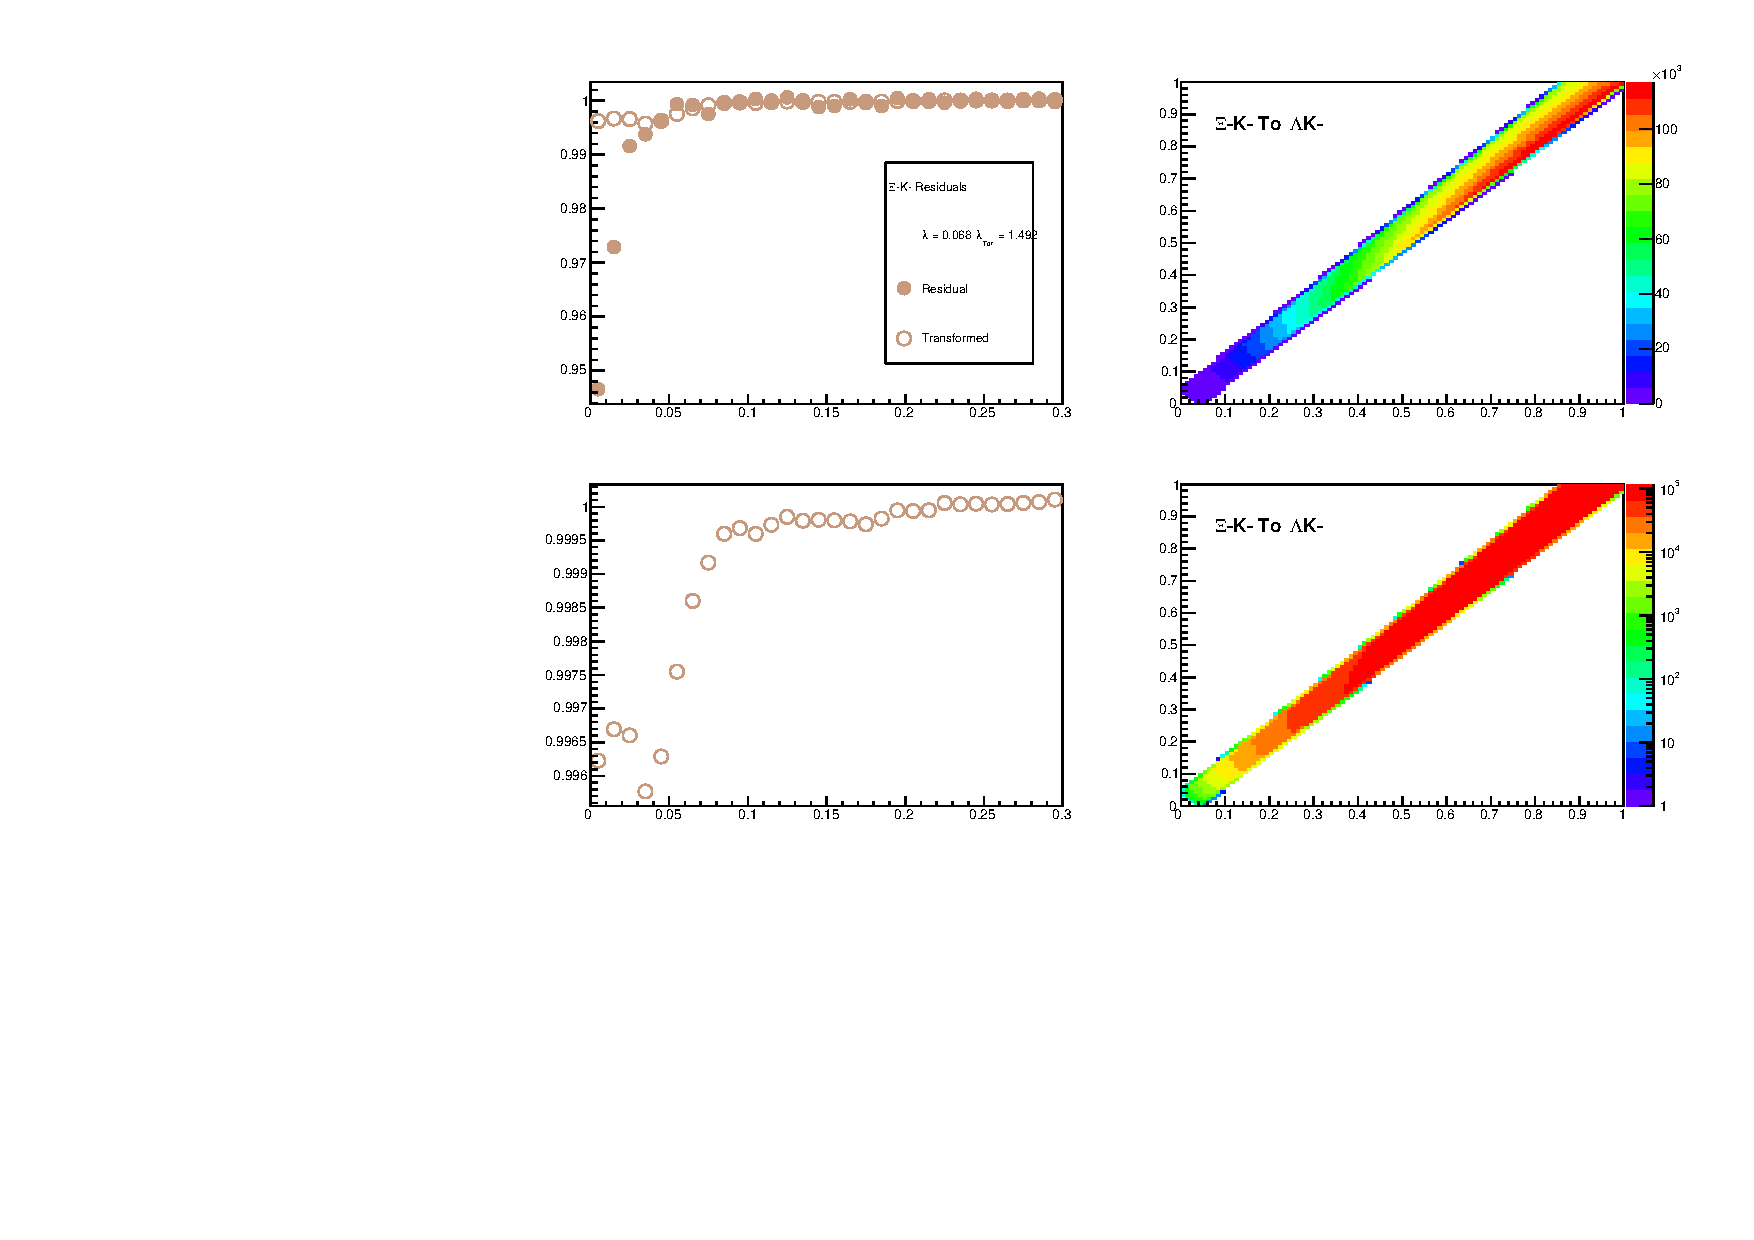
\includegraphics[width=\textwidth]{9_AdditionalFigures/Figures/Residuals/LamKchM/Residuals_LamKchM_0010_XiKchM_MomResCrctn_NonFlatBgdCrctn_ResidualsIncluded_UsingCoulombOnlyInterpCfs.pdf}
  \caption[Residuals: $\Xi^{-}$K$^{-}$ to $\Lambda$K$^{-}$ (0-10\% Centrality)]{Residuals: $\Xi^{-}$K$^{-}$ to $\Lambda$K$^{-}$ (0-10\% Centrality)}
  \label{fig:Res_LamKchM_0010_XiCKchM}
\end{figure}


\begin{figure}[h]
  \centering
  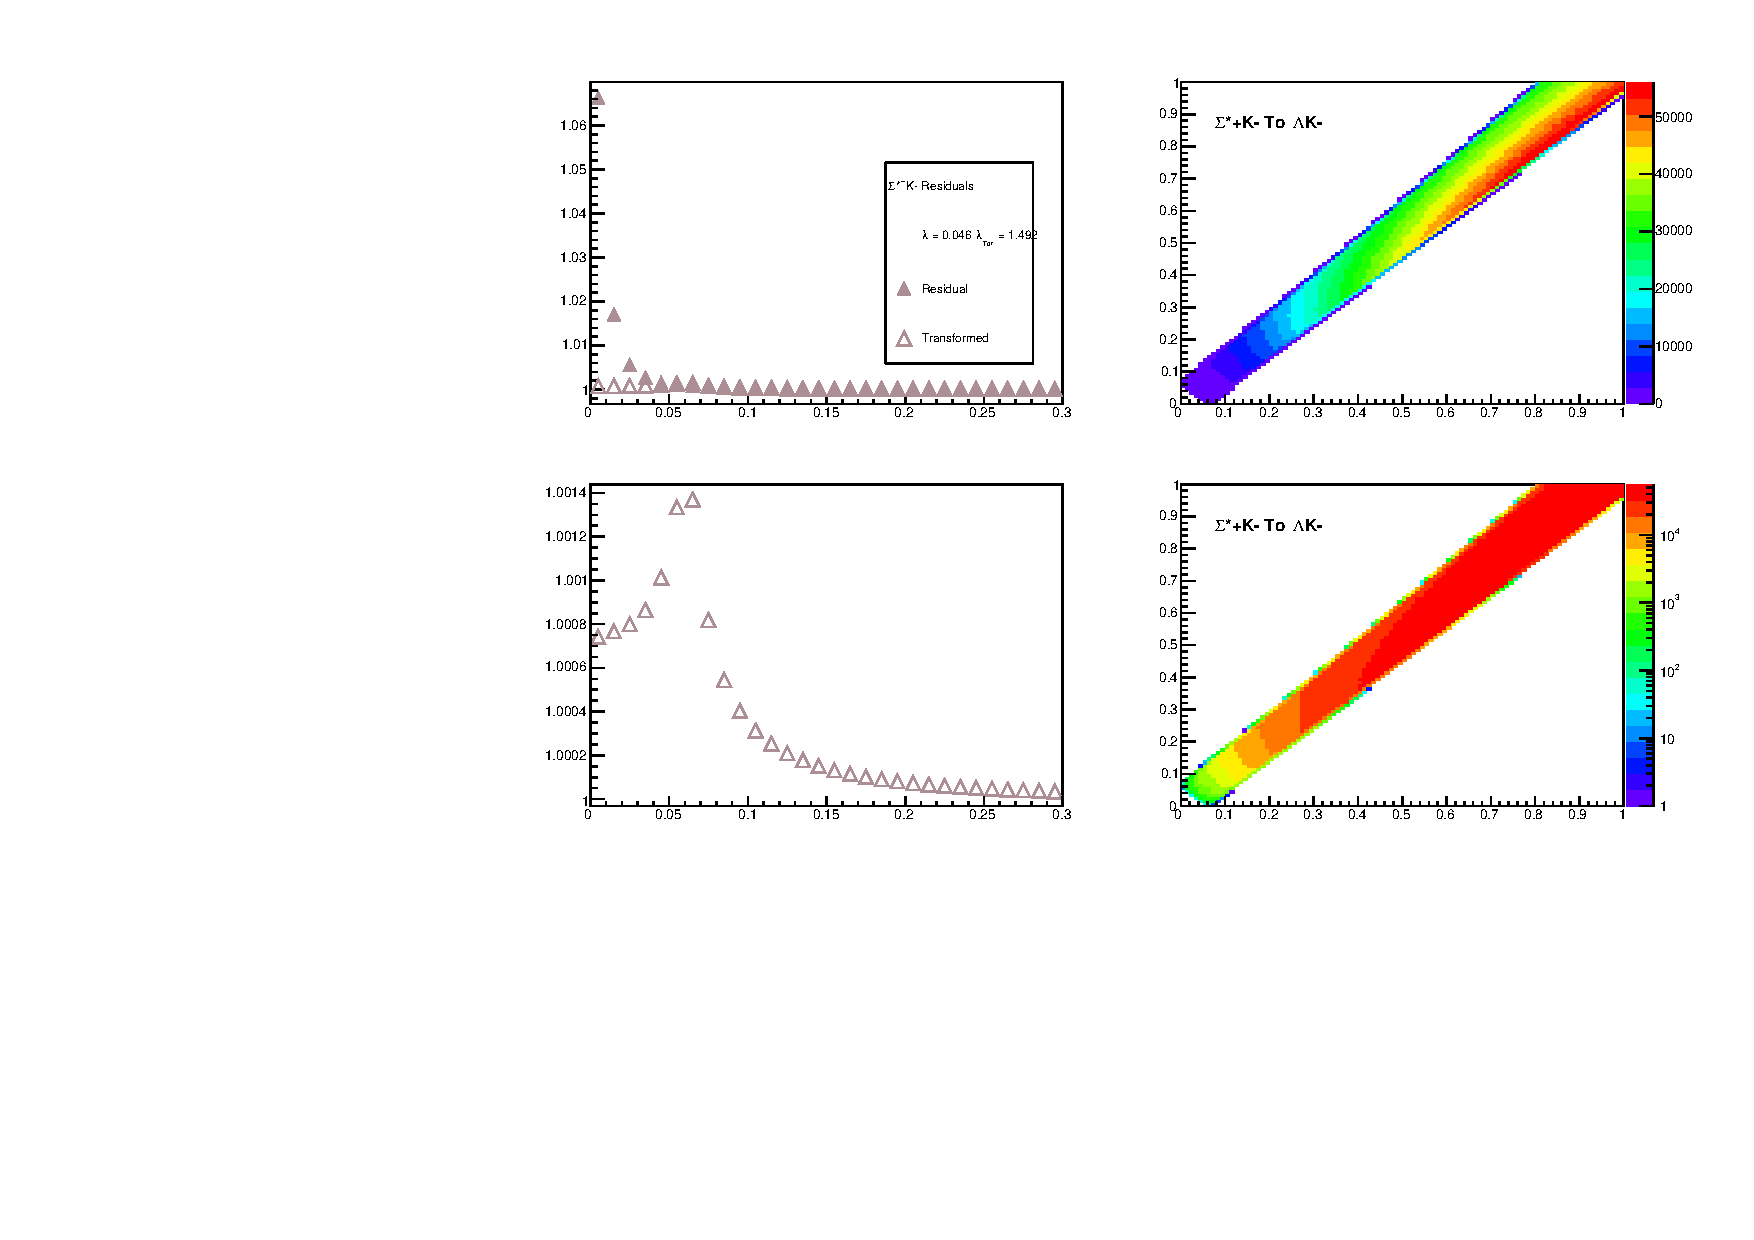
\includegraphics[width=\textwidth]{9_AdditionalFigures/Figures/Residuals/LamKchM/Residuals_LamKchM_0010_SigStPKchM_MomResCrctn_NonFlatBgdCrctn_ResidualsIncluded_UsingCoulombOnlyInterpCfs.pdf}
  \caption[Residuals: $\Sigma^{*+}$K$^{-}$ to $\Lambda$K$^{-}$ (0-10\% Centrality)]{Residuals: $\Sigma^{*+}$K$^{-}$ to $\Lambda$K$^{-}$ (0-10\% Centrality)}
  \label{fig:Res_LamKchM_0010_SigStPKchM}
\end{figure}

\begin{figure}[h]
  \centering
  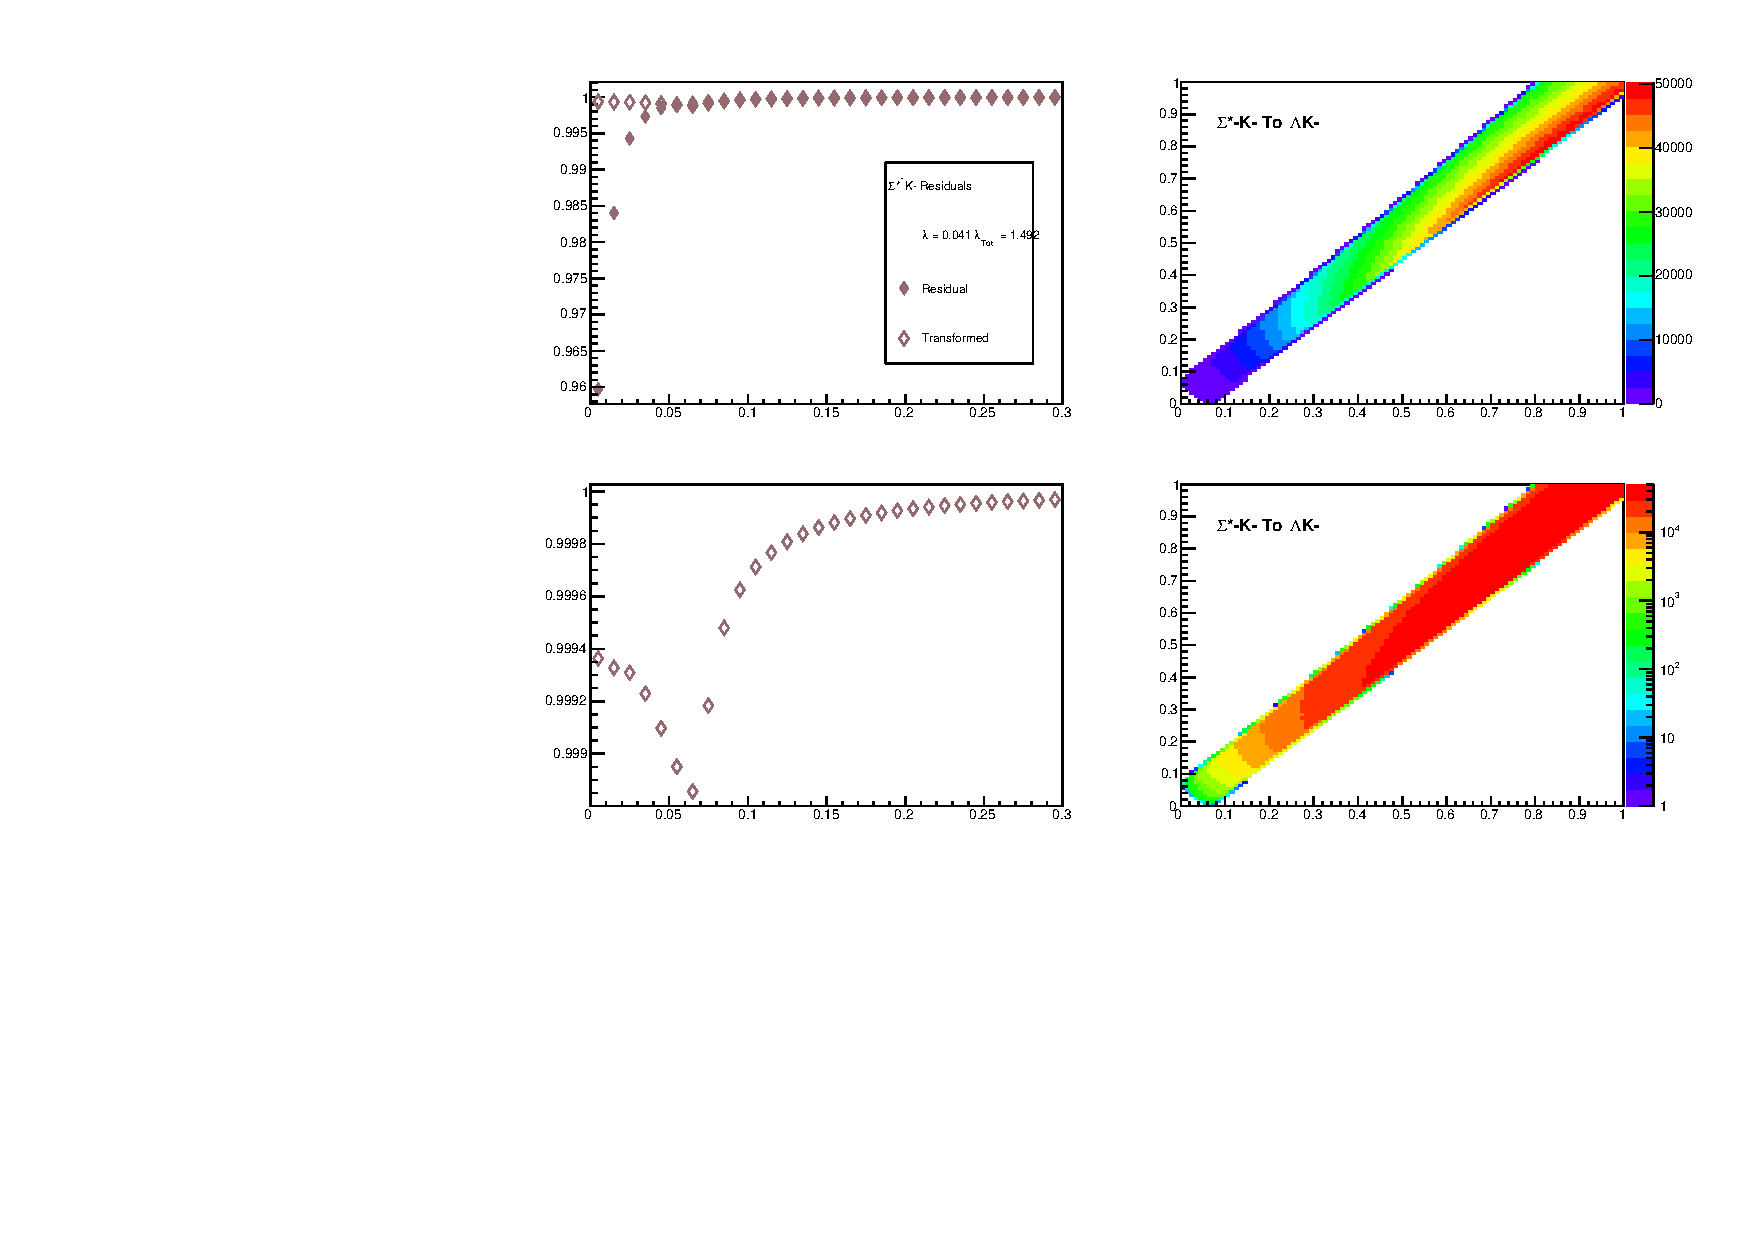
\includegraphics[width=\textwidth]{9_AdditionalFigures/Figures/Residuals/LamKchM/Residuals_LamKchM_0010_SigStMKchM_MomResCrctn_NonFlatBgdCrctn_ResidualsIncluded_UsingCoulombOnlyInterpCfs.pdf}
  \caption[Residuals: $\Sigma^{*-}$K$^{-}$ to $\Lambda$K$^{-}$ (0-10\% Centrality)]{Residuals: $\Sigma^{*-}$K$^{-}$ to $\Lambda$K$^{-}$ (0-10\% Centrality)}
  \label{fig:Res_LamKchM_0010_SigStMKchM}
\end{figure}

\begin{figure}[h]
  \centering
  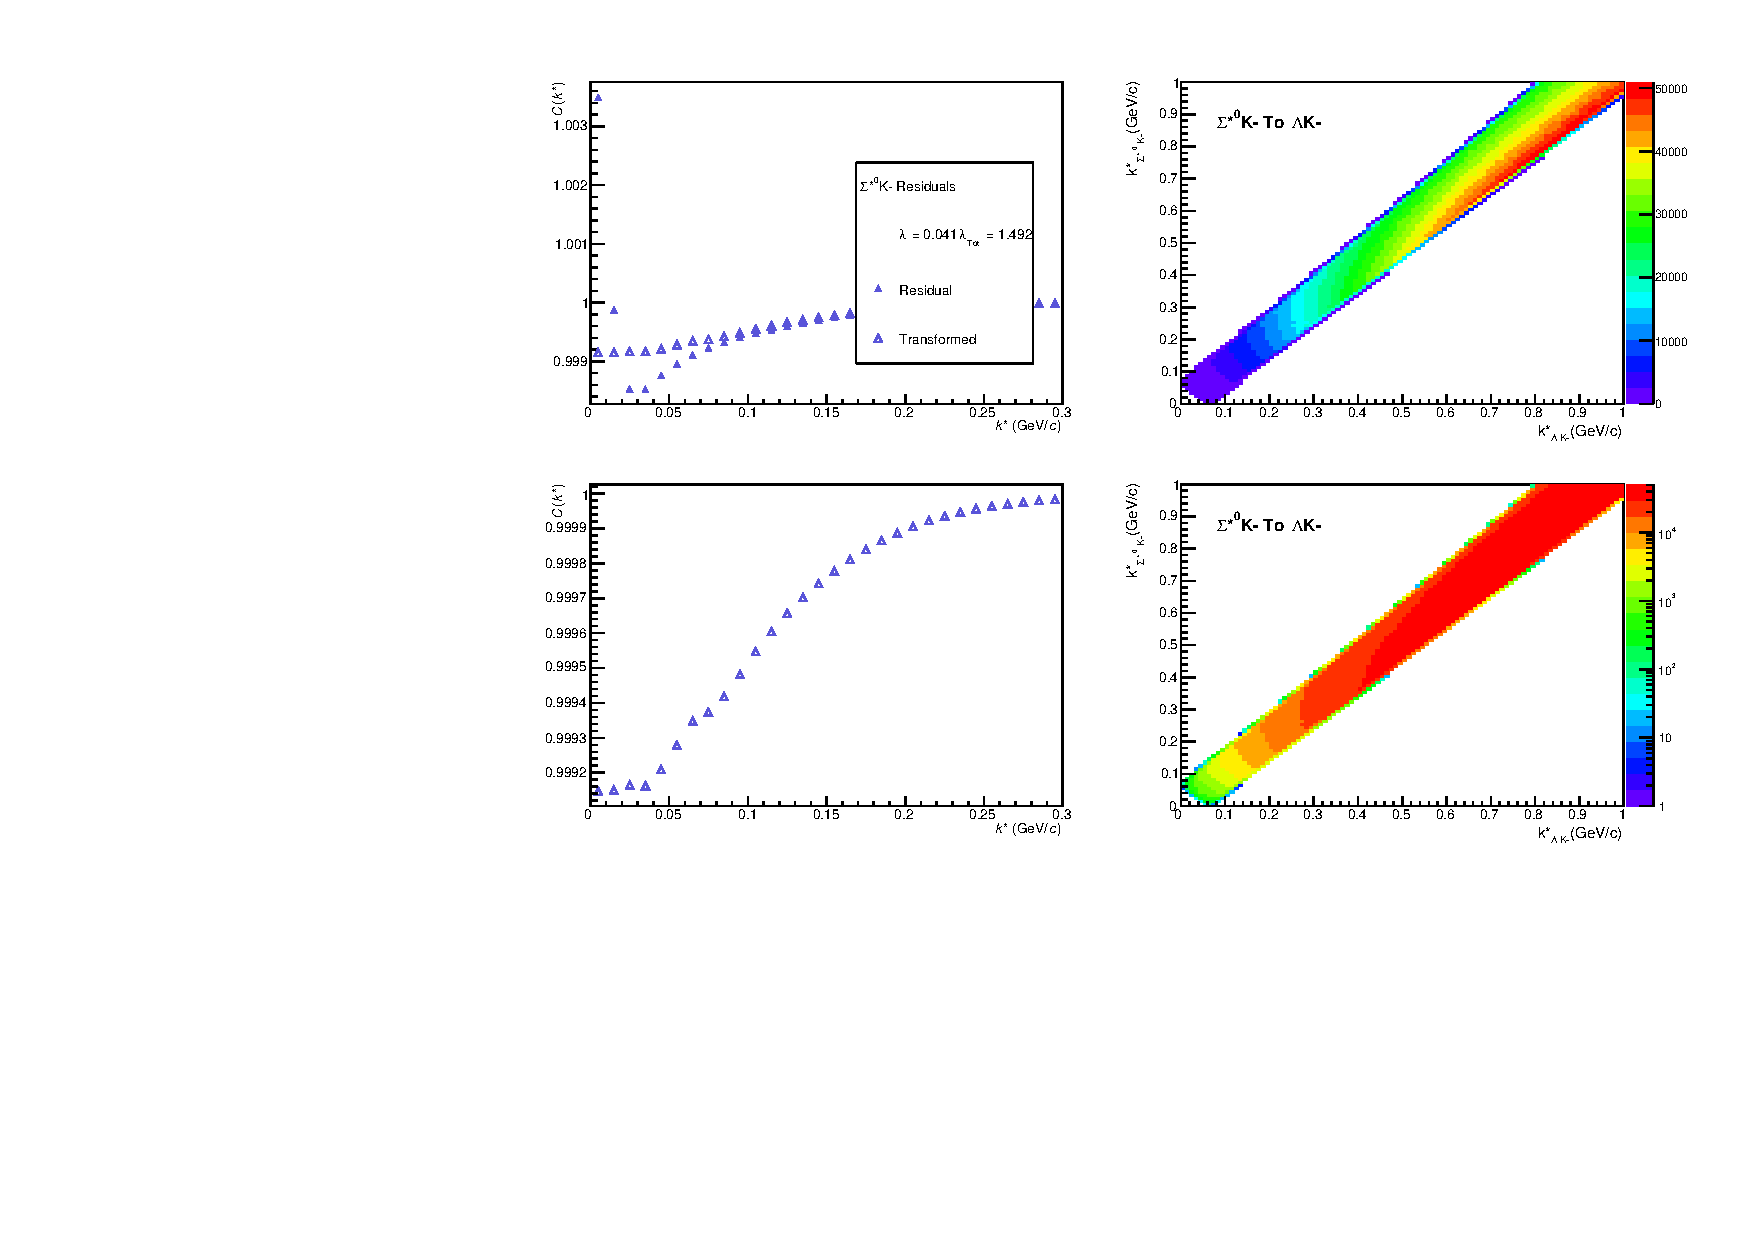
\includegraphics[width=\textwidth]{9_AdditionalFigures/Figures/Residuals/LamKchM/Residuals_LamKchM_0010_SigSt0KchM_MomResCrctn_NonFlatBgdCrctn_ResidualsIncluded_UsingCoulombOnlyInterpCfs.pdf}
  \caption[Residuals: $\Sigma^{*0}$K$^{-}$ to $\Lambda$K$^{-}$ (0-10\% Centrality)]{Residuals: $\Sigma^{*0}$K$^{-}$ to $\Lambda$K$^{-}$ (0-10\% Centrality)}
  \label{fig:Res_LamKchM_0010_SigSt0KchM}
\end{figure}


\begin{figure}[h]
  \centering
  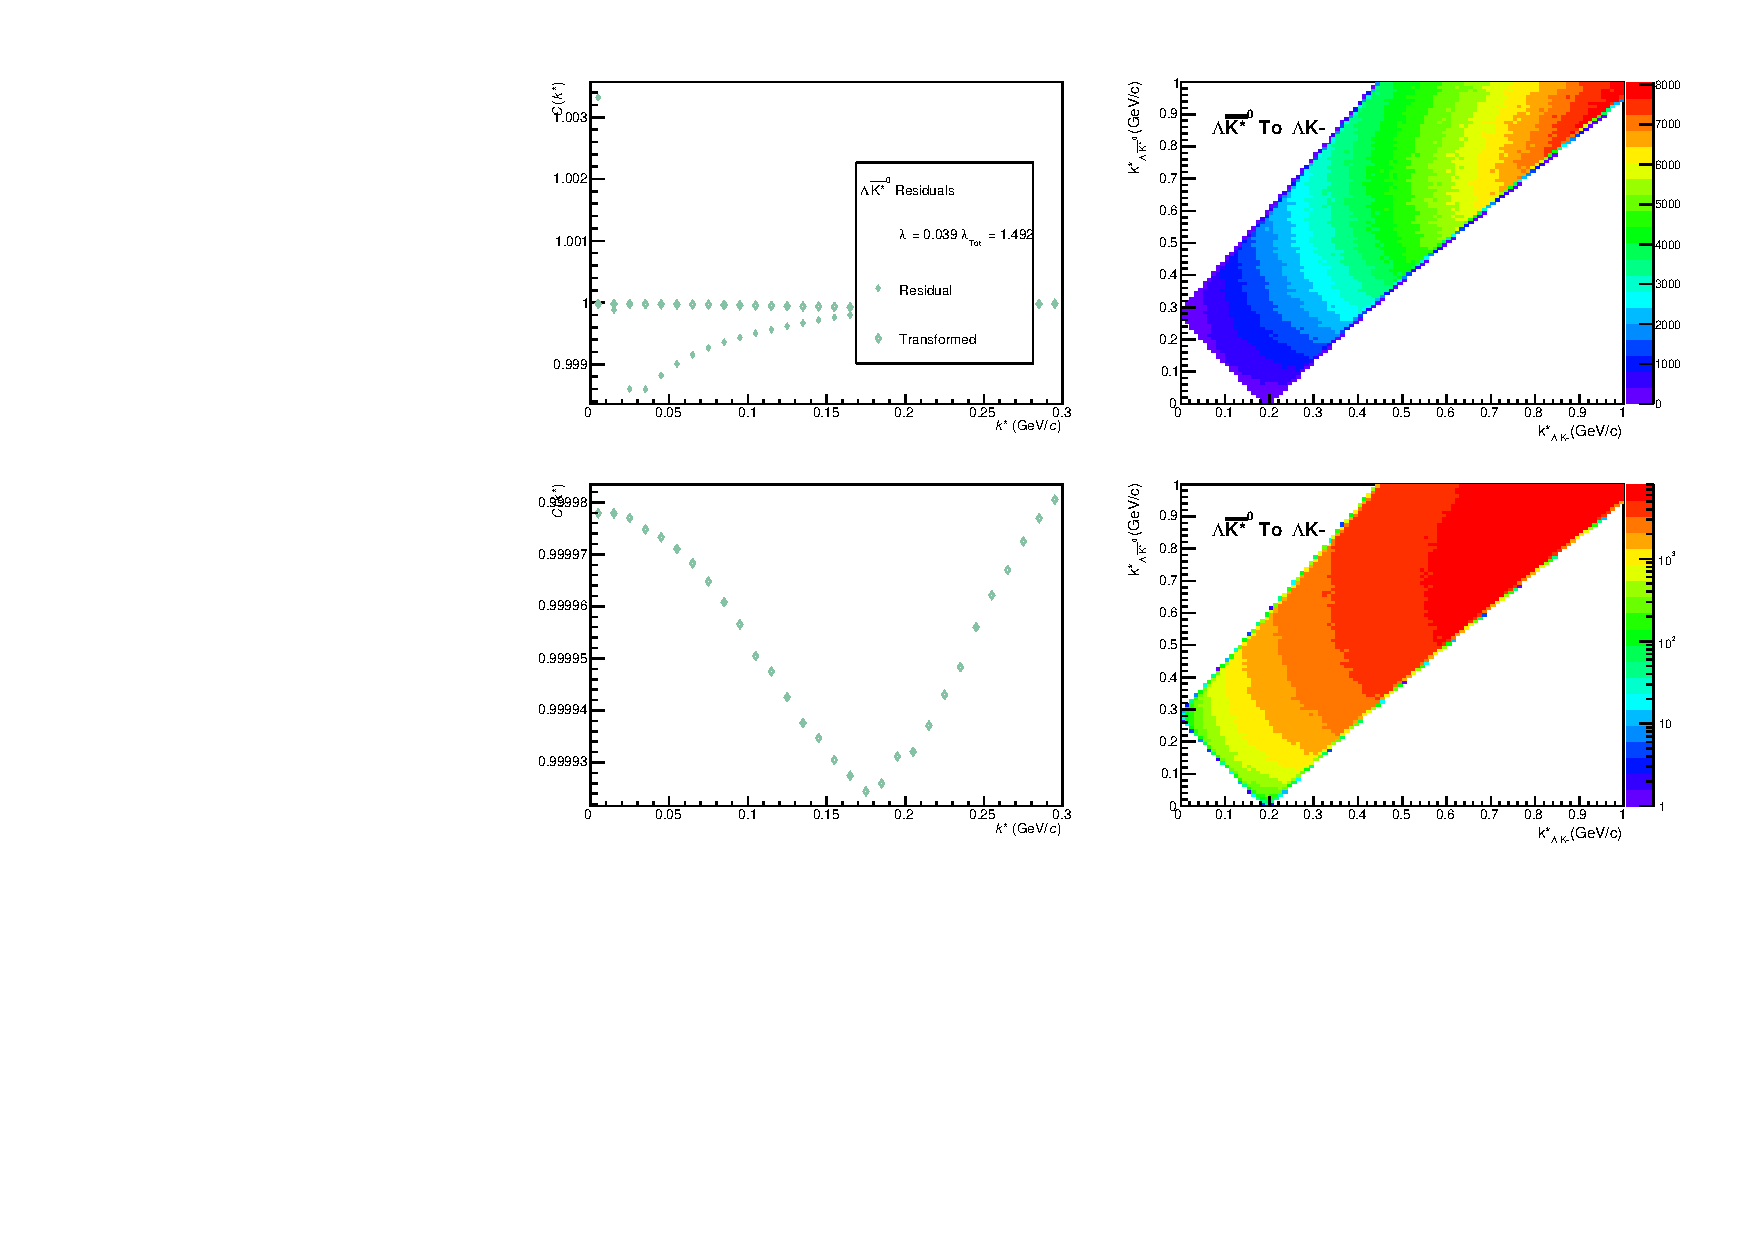
\includegraphics[width=\textwidth]{9_AdditionalFigures/Figures/Residuals/LamKchM/Residuals_LamKchM_0010_LamAKSt0_MomResCrctn_NonFlatBgdCrctn_ResidualsIncluded_UsingCoulombOnlyInterpCfs.pdf}
  \caption[Residuals: $\Lambda\bar{\mathrm{K}}^{*0}$ to $\Lambda$K$^{-}$ (0-10\% Centrality)]{Residuals: $\Lambda\bar{\mathrm{K}}^{*0}$ to $\Lambda$K$^{-}$ (0-10\% Centrality)}
  \label{fig:Res_LamKchM_0010_LamAKSt0}
\end{figure}


\begin{figure}[h]
  \centering
  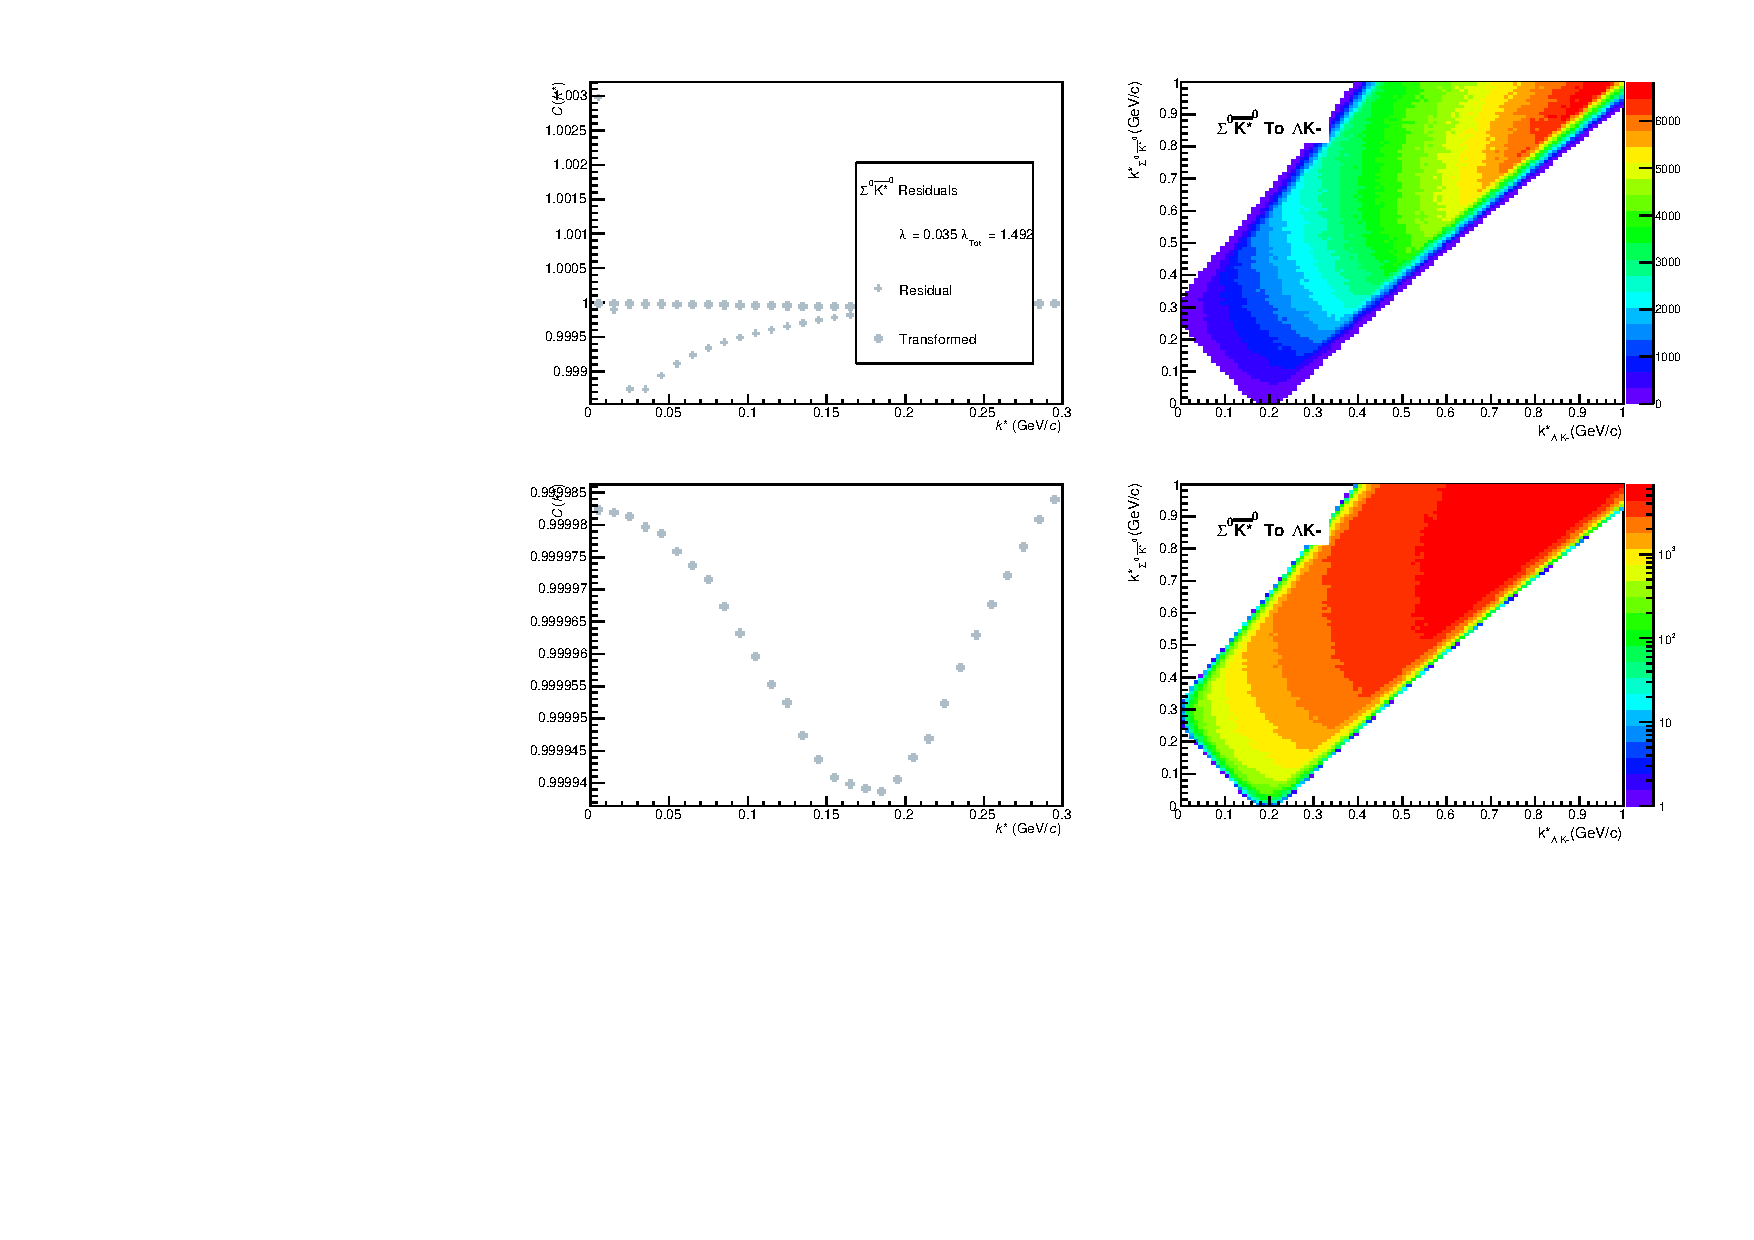
\includegraphics[width=\textwidth]{9_AdditionalFigures/Figures/Residuals/LamKchM/Residuals_LamKchM_0010_Sig0AKSt0_MomResCrctn_NonFlatBgdCrctn_ResidualsIncluded_UsingCoulombOnlyInterpCfs.pdf}
  \caption[Residuals: $\Sigma^{0}\bar{\mathrm{K}}^{*0}$ to $\Lambda$K$^{-}$ (0-10\% Centrality)]{Residuals: $\Sigma^{0}\bar{\mathrm{K}}^{*0}$ to $\Lambda$K$^{-}$ (0-10\% Centrality)}
  \label{fig:Res_LamKchM_0010_Sig0AKSt0}
\end{figure}


\begin{figure}[h]
  \centering
  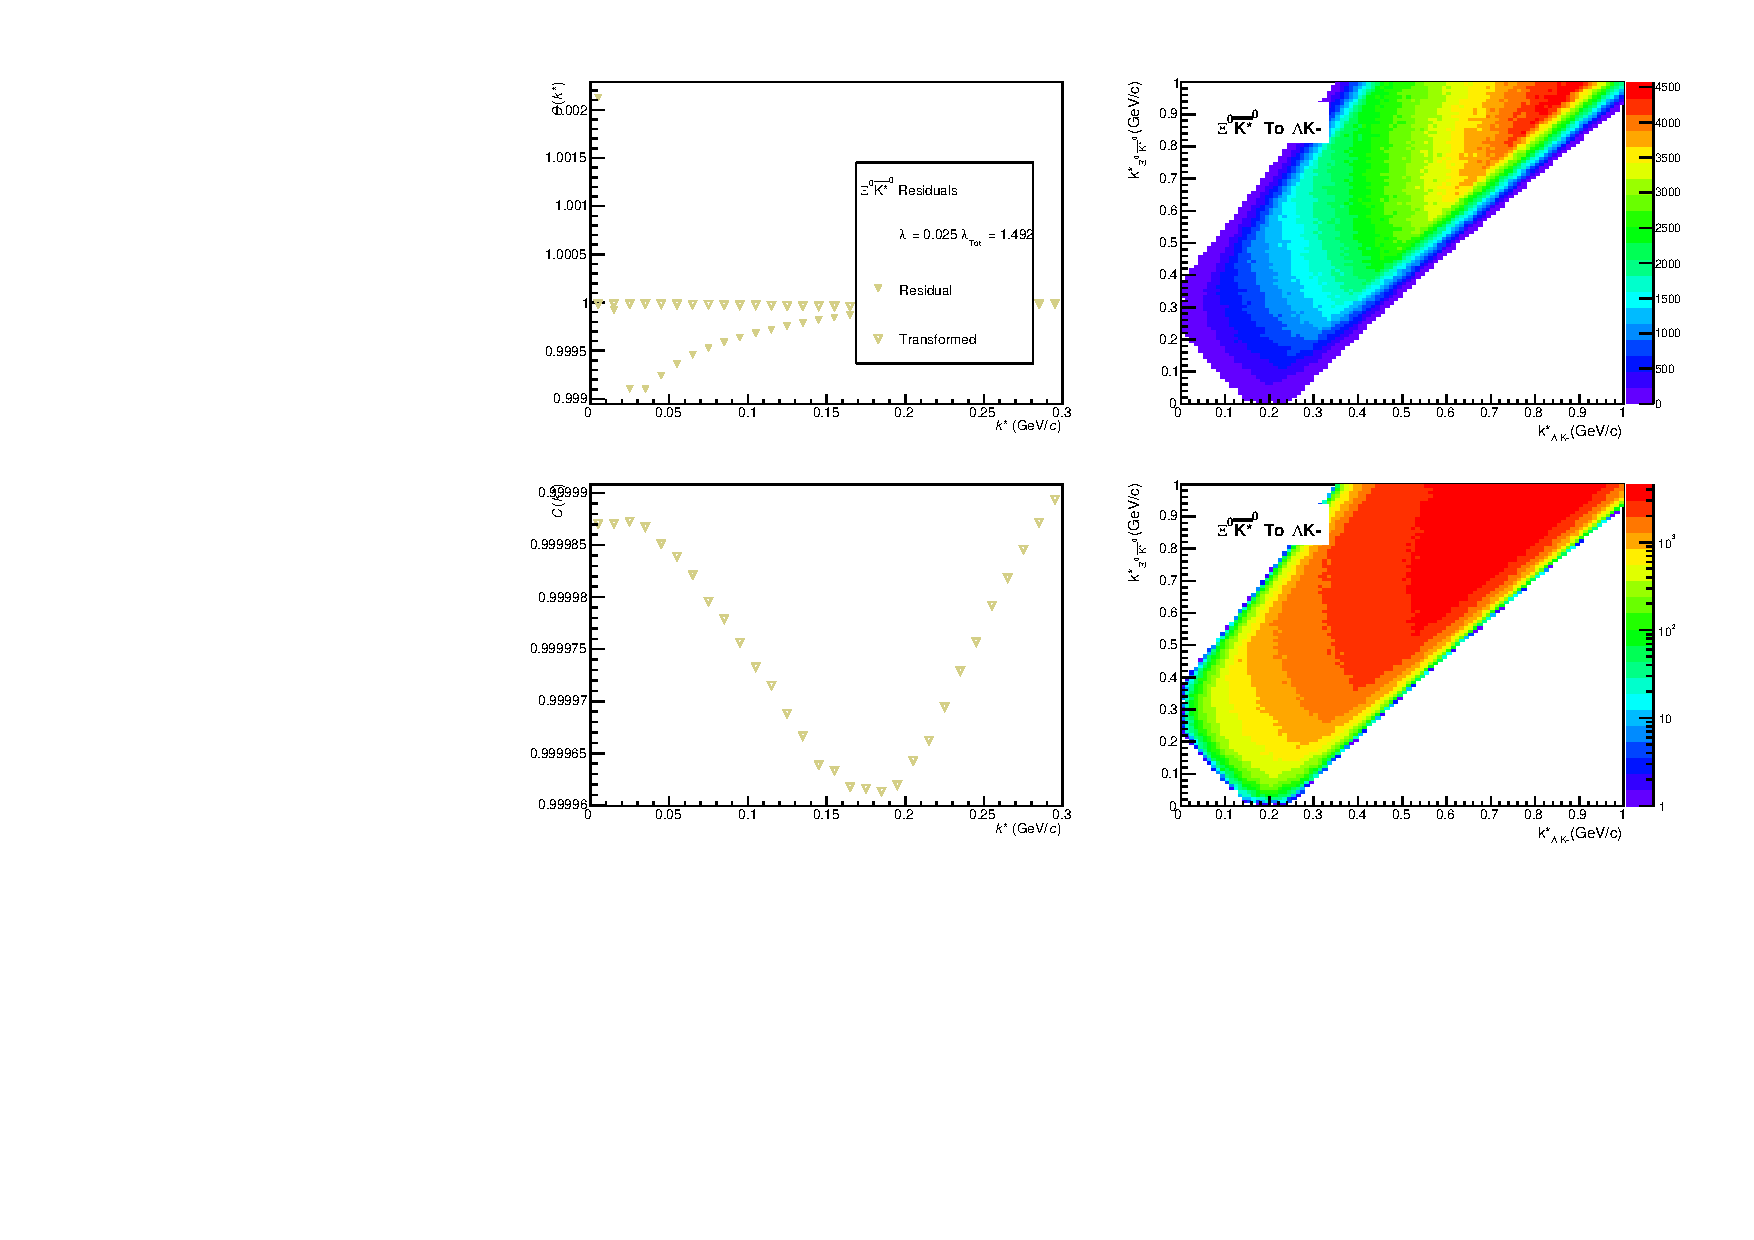
\includegraphics[width=\textwidth]{9_AdditionalFigures/Figures/Residuals/LamKchM/Residuals_LamKchM_0010_Xi0AKSt0_MomResCrctn_NonFlatBgdCrctn_ResidualsIncluded_UsingCoulombOnlyInterpCfs.pdf}
  \caption[Residuals: $\Xi^{0}\bar{\mathrm{K}}^{*0}$ to $\Lambda$K$^{-}$ (0-10\% Centrality)]{Residuals: $\Xi^{0}\bar{\mathrm{K}}^{*0}$ to $\Lambda$K$^{-}$ (0-10\% Centrality)}
  \label{fig:Res_LamKchM_0010_Xi0AKSt0}
\end{figure}

\begin{figure}[h]
  \centering
  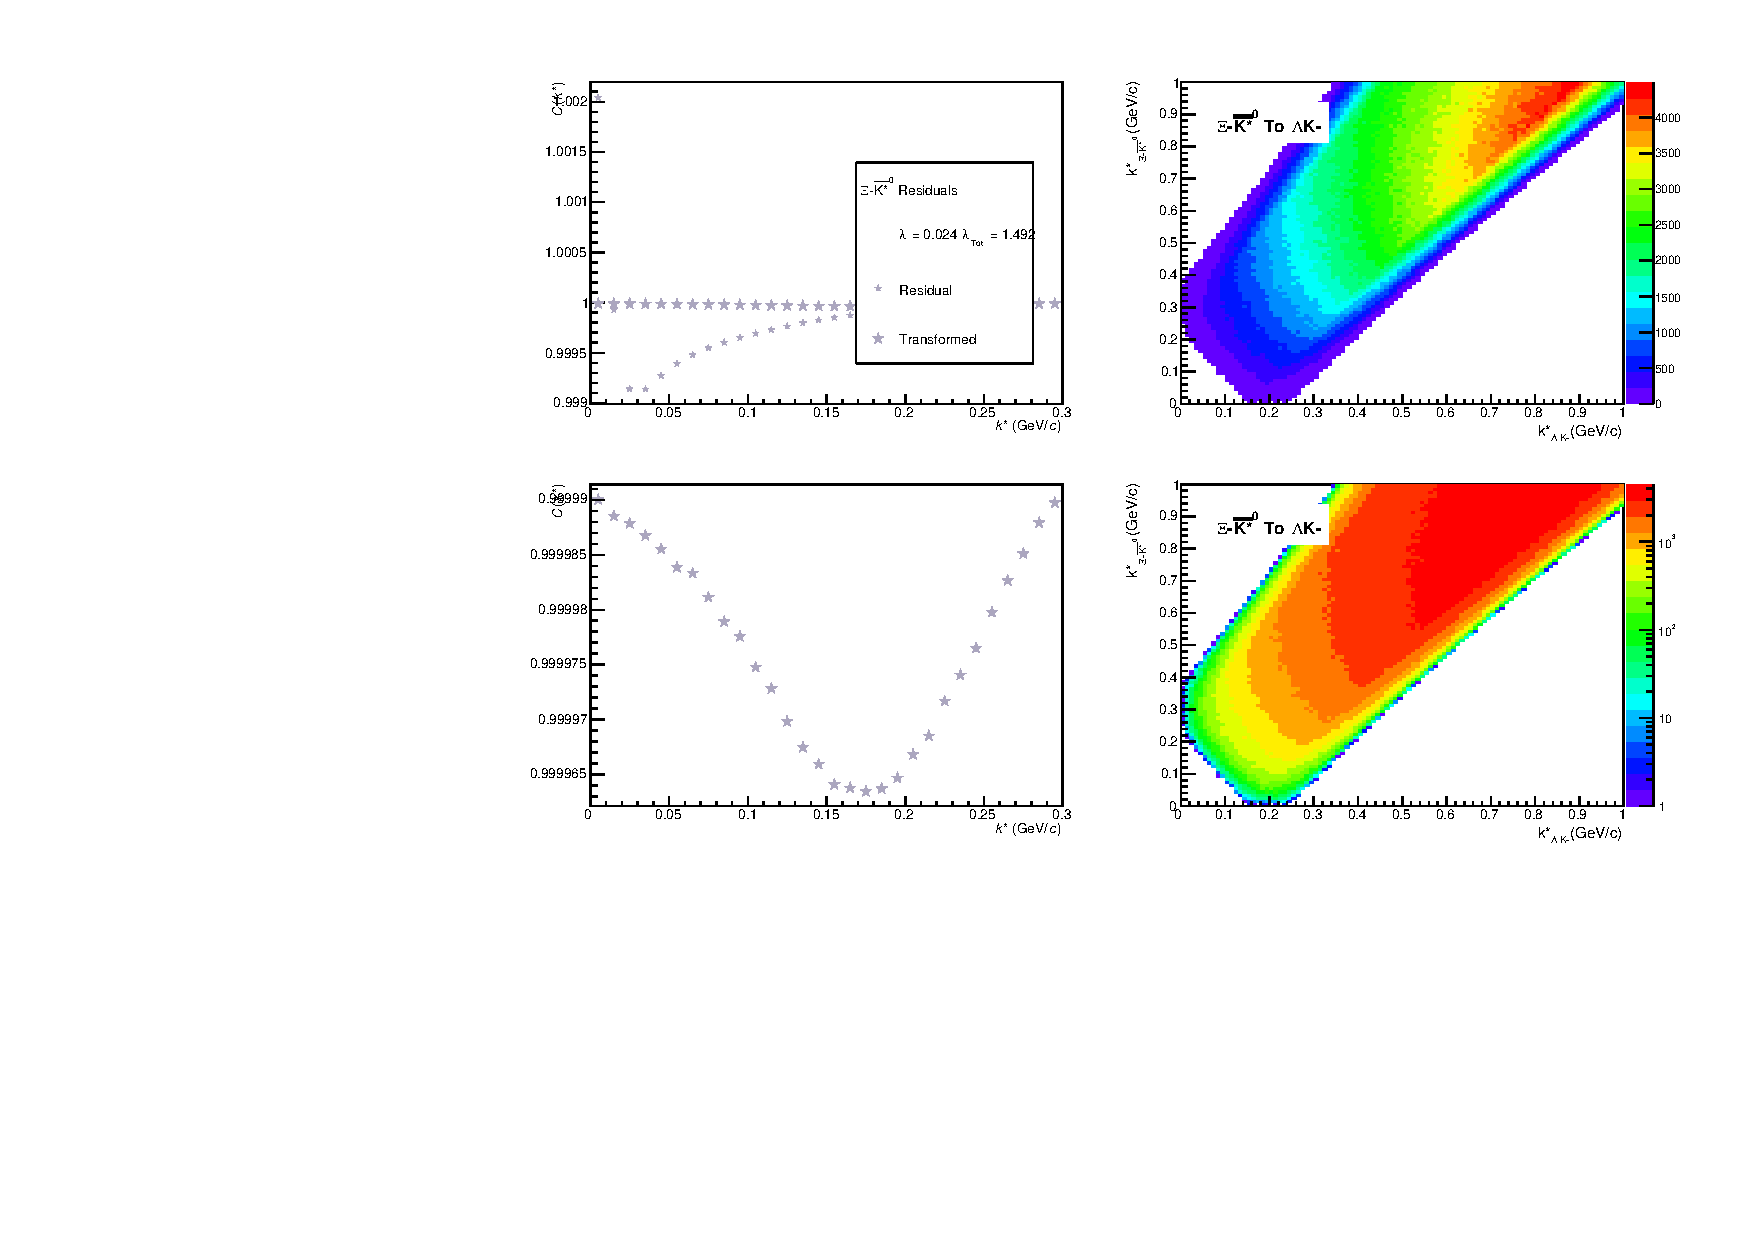
\includegraphics[width=\textwidth]{9_AdditionalFigures/Figures/Residuals/LamKchM/Residuals_LamKchM_0010_XiAKSt0_MomResCrctn_NonFlatBgdCrctn_ResidualsIncluded_UsingCoulombOnlyInterpCfs.pdf}
  \caption[Residuals: $\Xi^{-}\bar{\mathrm{K}}^{*0}$ to $\Lambda$K$^{-}$ (0-10\% Centrality)]{Residuals: $\Xi^{-}\bar{\mathrm{K}}^{*0}$ to $\Lambda$K$^{-}$ (0-10\% Centrality)}
  \label{fig:Res_LamKchM_0010_XiCAKSt0}
\end{figure}

\end{document}